\documentclass[11pt]{article}

% Review version: line numbers, anonymized. For the camera-ready
% version, change \usepackage[review]{acl} to \usepackage{acl}.
\usepackage[review]{acl}

\usepackage{times}
\usepackage{latexsym}
\usepackage[T1]{fontenc}
\usepackage[utf8]{inputenc}
\usepackage{microtype}
\usepackage{inconsolata}
\usepackage{graphicx}

% Added for this paper: math, tables, algorithms.
\usepackage{amsmath}
\usepackage{amssymb}
\usepackage{booktabs}
\usepackage{algorithm}
\usepackage{algpseudocode}

\title{Code Localization as Sequential Set-Coverage: \\
       A Trainable Multi-Round Scaffolding for Small LLMs}

% Anonymized for review. Restore the full author block for the
% camera-ready version.
\author{Anonymous ACL submission}

\begin{document}
\maketitle

\begin{abstract}
Before a coding agent can fix a GitHub issue, it must localize the files and functions to change; a mistake here cannot be undone by any later reasoning. Strong localization scaffoldings such as OpenHands and SWE-Agent are built for long contexts and large models, so the open 7--14B code models most teams can run overflow a 32K-token budget before the search ends. Training small models is no easier: a multi-step agent yields only a sparse terminal reward, forcing expensive reinforcement learning. We present a multi-round localization scaffolding that removes both barriers. The agent refines a fixed-length candidate list over rounds, each round inspecting a bounded window of ranked nodes and their neighborhood on a code graph, so per-call token cost stays roughly constant. The round structure also exposes a dense per-round target: under potential-based shaping, the per-round signal telescopes to end-to-end recall@$L$. The agent therefore trains by ordinary supervised fine-tuning---a weighted cross-entropy with a differentiable coverage term---rather than sparse-reward RL. This recasts localization from ranking to sequential set-coverage on a code graph. Trained this way, small open models become competitive with GPT Codex~5.3 under the same scaffolding, and a 30B model matches open-ended OpenHands agents at a fraction of the token cost, on SWE-Bench Lite, SWE-Bench Verified, and the multilingual SWE-PolyBench.
\end{abstract}

\section{Introduction}
\label{sec:intro}

LLM coding agents increasingly resolve real GitHub issues by
editing a repository directly, and benchmarks such as SWE-Bench
now track how often they succeed \citep{jimenez2024swebench}. A
patch can only be correct, however, if it changes the right
code. Before any edit, the agent must identify the files and
functions an issue actually touches, the step known as
\emph{code localization}. This step is decisive and largely
unrecoverable: once a wrong location enters the agent's editable
context, the repair stage reasons over the wrong code, and no
later reasoning recovers the correct patch
\citep{jimenez2024swebench, yang2024sweagent}. \citet{xia2024agentless}
drop agentic interaction and resolve issues with a fixed
localize-then-repair pipeline, crediting much of their accuracy
to a hierarchical localization phase, and methods that improve
the localization stage report corresponding gains in end-to-end
resolution \citep{sohrabizadeh2025nemotroncortexa}. Localization
is therefore not a preprocessing convenience but the step that
determines how well downstream repair can perform.

% Yet localizing well is hard: a real repository holds thousands
% of files joined by tangled import, call, and inheritance edges,
% while an issue report describes symptoms in natural language
% that can sit far from the code that must change. 
Current systems close this gap in four ways. Reinforcement learning methods
train the search policy itself: RepoSearcher pairs
tool-integrated RL with rejection-sampled supervised
fine-tuning \citep{ma2025tooltrain}, and SWE-RL scales RL over
open software-evolution data \citep{wei2025swerl}.
General-purpose agent scaffoldings give a capable LLM an
open-ended action space with shell access, as in SWE-Agent and
OpenHands \citep{yang2024sweagent, wang2025openhands}.
Graph-exploration agents such as LocAgent let an LLM traverse a
repository code graph, hopping freely between related code units
\citep{chen2025locagent}. Dense retrieval methods skip the agent
altogether: SWERank scores code units with a bi-encoder
retriever and a listwise LLM scorer
\citep{reddy2025sweranksoftwareissuelocalization}.

The first three families pay for accuracy in tokens, and none of
them bounds the cost. An RL agent, an open-ended scaffold, and a
graph explorer all keep issuing tool calls and appending
observations until they choose to stop, so a localization
trajectory grows without a predictable ceiling. Under an
OpenHands-style scaffolding, a single localization run can
exceed 131K tokens. A model with a
long context window and ample compute absorbs that cost; the
open 7--14B code models most teams can realistically run do not.
A Qwen-class coder with a 32K-token window overflows before the
search terminates. Reinforcement learning compounds the problem:
a multi-step episode returns only a sparse terminal reward, so
adapting a small model to it takes many long and expensive
rollouts. Dense retrieval is the one cheap option, but a
single-step, order-centric ranker cannot revisit a discarded
candidate or follow a structural edge, so it leaves the
sequential, graph-structured side of the problem untouched. No
existing method is at once bounded in token cost at inference
and cheap enough to train on a small open model.

% ============================================================
% OUTLINE -- Introduction paragraph 4 (CONTRIBUTIONS) -- TO WRITE
% Close on explicit contributions + a one-line results preview,
% then transition to Sec. 2. Draft pending user decision on the
% contribution list.
%   C1  a multi-round, bounded-context localization scaffolding
%       for small code LLMs;
%   C2  a telescoping result: the dense per-round target shares
%       its optimum with end-to-end recall@L (no myopia gap),
%       converting a sparse-reward multi-step RL problem into
%       supervised learning;
%   C3  a supervised objective -- weighted BCE + a differentiable
%       coverage term -- provably co-optimal with recall@L, and
%       the set-coverage reframing it rests on;
%   C4  results: small open models competitive with GPT Codex
%       5.3 under the same scaffolding; Qwen-30B competitive
%       with OpenHands at a fraction of the token cost; on
%       SWE-Bench Lite, SWE-Bench Verified, and SWE-PolyBench.
% ============================================================

\input{sections/2_Related_Work}
\section{Method}
\label{sec:method}

% ============================================================
% OUTLINE -- Method            target: ~1.5-1.7 pages (the core)
% Spine: setup -> scaffolding (bounded cost) -> dense per-round
% target (telescoping => supervised, not RL) -> the loss.
%
% Notation (use consistently paper-wide):
%   G = (V,E)  code graph; edges = contains/call/import/co-change
%   Y*         gold set of code units that must change
%   L          the fixed-length returned list; recall@L the metric
%   K          window size: ranked candidates revealed per round
%   P_r        per-round candidate pool
%   Phi_r      secured-gold potential
% Display equations in the body: the telescoping identity, the
% weighted BCE, the coverage term. Three equations max.
% ============================================================

\subsection{Problem Setup}
\label{sec:setup}
% - Repository R, natural-language issue q. A code graph
%   G = (V,E): nodes are code units (file / class / function),
%   edges are structural relations (contains, call, import,
%   co-change).
% - Task: recover the gold set Y* of units that must be modified.
% - Metric: recall@L over a fixed-length returned list L.
% - Frame the task as SET RECOVERY, not ranking -- this framing
%   is exactly what the objective in 3.4 is built to match.
%   (~0.2-0.25 page)

\subsection{Multi-Round Localization Scaffolding}
\label{sec:scaffold}

The scaffolding processes a single issue $q$ over $R$ rounds. A
retriever (dense, lexical, or their union) returns a ranked
list of code units, and each round consumes the next $K$ unseen
entries of that list. At the start of round $r$, the
scaffolding holds three pieces of state: the current returned
list $L_{r-1}$ (initialised to $\emptyset$ at $r{=}0$), the set
of node identifiers $\mathcal{S}_{r-1}$ already shown to the
model, and an offset $rK$ into the ranked list. The loop
terminates when the ranked list is exhausted or a maximum
number of rounds $R_{\max}$ is reached. An optional
confident-stop hook is left for the RL stage
(Section~\ref{sec:conclusion}); the supervised training of
Section~\ref{sec:objective} does not predict it, so a
trajectory always runs to $R_{\max}$ or exhaustion.

Each round combines a bounded window of newly-ranked candidates
with a bounded graph-neighborhood expansion, then refines $L$;
Figure~\ref{fig:scaffold} sketches the loop.

\begin{figure}[t]
\centering
% TODO: replace with the multi-round scaffolding diagram.
\fbox{\rule{0pt}{2.4cm}\rule{0.9\columnwidth}{0pt}}
\caption{The multi-round localization scaffolding. Each round
consumes a bounded window of $K$ ranked candidates, expands
neighborhoods around $C$ seed centers via bounded BFS on the
code graph, and refines a fixed-length returned list $L_r$.
Per-call token cost stays roughly constant across rounds.}
\label{fig:scaffold}
\end{figure}

\paragraph{Window.}
The scaffolding pulls the next $K$ unseen entries of the ranked
list starting at offset $rK$, skipping any node already in
$\mathcal{S}_{r-1}$. We denote this window $W_r$. If $W_r$ is
empty the round terminates the loop.

\paragraph{Step A: seed-center selection.}
A single model call selects $C$ seed centers from $W_r$, i.e.\
nodes whose graph neighborhoods are most likely to contain
unseen gold units. If the model returns fewer than $C$ valid
identifiers we pad with the top-ranked nodes of $W_r$ not yet
returned, so Step~A always emits exactly $C$ centers.

\paragraph{Step B: neighborhood expansion.}
For each of the $C$ centers, the scaffolding runs a depth-$d$
BFS along structural edges of the code graph (\textit{contains}
by default; ablations in Section~\ref{sec:ablation} cover the
four edge types). The neighbors are filtered to the next $N$
unseen entries of the ranked list, so the candidate set the
model sees stays bounded. A model call per center then selects
the subset of these neighbors that must be modified, and the
union across centers, $\mathcal{N}_r$, is deduplicated.

\paragraph{Step C: list refinement.}
A final model call sees the issue $q$, the current list
$L_{r-1}$, the window $W_r$, and the deduplicated set
$\mathcal{N}_r$, and selects $L$ identifiers from
$L_{r-1} \cup W_r \cup \mathcal{N}_r$ to form $L_r$. The
scaffolding then records the newly-shown identifiers, advances
the offset, and continues.

Three properties of this loop matter for what follows.
\emph{First}, every model call sees only $W_r$, a single
neighborhood, or the deduplicated round pool, so the per-call
token cost is roughly constant across rounds; a 32K context
comfortably absorbs each call regardless of how many rounds the
trajectory uses. \emph{Second}, the loop offers a natural
ablation: removing Steps~A and~B reduces it to a pure
window-refine loop and isolates the contribution of graph
exploration. \emph{Third}, $L_r$ at any round is a valid
prediction, so the round structure exposes a per-round
potential that we develop into a training target in the next
section.

\subsection{A Dense, Recall-Aligned Per-Round Target}
\label{sec:telescope}
% - Define the secured-gold potential  Phi_r = |Y* intersect L_r|.
% - Per-round signal  r_r = (Phi_r - Phi_{r-1}) / D, with
%   D = |Y* intersect candidates|  =  (gold added - gold dropped)/D.
% - EQUATION (telescoping):  sum_r r_r = (Phi_R - Phi_0)/D
%   = recall@L(L_final) - recall@L(L_0).
% - THEOREM (state here, proof -> Appendix A): by potential-
%   based reward shaping \citep{ng1999policy}, shaping with a
%   state potential leaves the optimal policy invariant; hence
%   the dense per-round objective and sparse end-to-end
%   recall@L share the same optimum -- there is no myopia gap.
% - IMPLICATION (the load-bearing sentence): the per-round
%   optimum is closed-form, so training needs no policy
%   gradient; supervised learning on the per-round target is
%   denser, more stable, and cheaper than RL on the same signal.
%   (~0.3-0.35 page)

\subsection{Supervised Training Objective}
\label{sec:objective}
% - Per round build the pool P_r = L_{r-1} U window_r; labels
%   y_j = 1[j in Y*].
% - Scoring without a new head: use the model's own yes/no
%   token logits, s_j = logit(yes) - logit(no), p_j = sigma(s_j).
%   Zero new parameters; LoRA-friendly; avoids the cold-start
%   failure of a randomly-initialized head.
% - EQUATION (weighted BCE): the main term; its optimum is
%   "every gold scored above every non-gold", which yields a
%   max-coverage top-L.
% - EQUATION (coverage term L_cov): a differentiable, listwise,
%   permutation-invariant surrogate for covering the whole gold
%   set; it never penalizes gold-vs-gold order.
% - Total objective: L = L_bce + lambda * L_cov.
% - State the guarantee scope: exact recall@L co-optimality
%   holds at w+ = w- = 1; an asymmetric w+ > w- is a class-
%   imbalance / "dropping gold is worse" heuristic -- report it
%   as a tuning choice, not part of the theorem. lambda = 0 is
%   the ablation baseline.
% - Top-L selection is inference-only and never differentiated.
% - One sentence: stages are trained densest-signal-first
%   (curriculum); full staging details -> Appendix B.
%   (~0.45-0.5 page)

\section{Experiments}
\label{sec:experiments}

% ============================================================
% OUTLINE -- Experiments          target: ~1.1-1.25 pages
% Claims to land, in order:
%   (1) fine-tuning with the scaffolding helps (vs un-finetuned);
%   (2) small / open models become competitive with GPT Codex
%       5.3 under the SAME scaffolding;
%   (3) Qwen-30B is competitive with open-ended OpenHands at a
%       fraction of the token cost;
%   (4) the coverage term helps (lambda = 0 vs lambda > 0);
%   (5) the margin widens as the gold set grows / disperses.
% RESULTS ARE PARTIAL / IN PROGRESS -- scaffold the tables with
% placeholders and fill exact numbers before submission.
% ============================================================

\subsection{Setup}
\label{sec:setup-exp}

\paragraph{Datasets.}
The scorer is trained on a fixed subset of $5{,}000$ issues drawn
from the SWE-Bench train split \citep{jimenez2024swebench} and
evaluated on SWE-Bench Verified \citep{jimenez2024swebench} ---
the human-verified subset restricted to issues with unambiguous
patches --- and SWE-PolyBench \citep{chaudhari2025spider}, a
multilingual SWE-Bench-style benchmark spanning Python, Java,
JavaScript and TypeScript. Across all three splits we recover the
ground-truth function set $G_i$ from the PR commit that resolved
issue $i$: every function whose body the patch modifies is treated
as gold. Group construction and negative sampling at training time
follow Appendix~\ref{app:details}.

\paragraph{Backbones and baselines.}
The scorer is fine-tuned from Qwen2.5-Coder-3B-Instruct
\citep{hui2024qwen25codertechnicalreport}. As un-fine-tuned
reference points under the same scaffolding we report
Qwen2.5-Coder-14B-Instruct, Qwen3-Coder-30B-A3B-Instruct
\citep{yang2025qwen3}, and GPT-5.3
Codex\footnote{OpenAI's \texttt{gpt-5.3-codex} coding model,
accessed via the OpenAI API in 2025; the exact snapshot
identifier and access date will be pinned in the camera-ready
version.}. The first-stage retriever is either SWERankEmbed-Large
\citep{reddy2025sweranksoftwareissuelocalization} (dense) or BM25
(lexical), in both cases truncated to a top-$N$ pool with
$N{=}500$. The zero-shot retriever output and the un-fine-tuned
scorer under the same scaffolding act as ablation baselines.

\paragraph{Decoding and reproducibility.}
All scorer and agent calls use temperature $0$ and the API
default for top-$p$. Decoding is therefore deterministic up to
backend non-determinism, and rerunning a configuration on the
same inputs shifts Recall@$5$ by less than $1$ percentage point
in our measurements. Reported numbers are from single runs;
seeds and prompt templates are fixed across rows of a given
table to keep cross-row differences attributable to the
scaffolding rather than to sampling.

\subsection{Main Results}
\label{sec:main-results}

Table~\ref{tab:verified} reports $\text{Recall}@5$ on SWE-Bench
Verified ($N{=}500$) for the zero-shot retrievers, the
un-fine-tuned baselines, and our fine-tuned scorer, under both
first-stage retrievers. The block labelled \emph{w/o graph} is the
ablation in which Step~B is disabled (Section~\ref{sec:scaffold}),
so the loop reduces to window-only refinement; the \emph{full} block
runs the complete three-step round.

\begin{table*}[t]
\centering
\small
\setlength{\tabcolsep}{5pt}
\renewcommand{\arraystretch}{1.05}
\caption{Retrieval performance on SWE-Bench Verified
($N{=}500$). $\text{Recall}@5$ is reported separately under a
dense (SWERankEmbed-Large) and a lexical (BM25) first-stage
retriever. Token consumption is the total tokens per issue
(tokens/call $\times$ \#calls), averaged across the two
retrievers.
$^{*}$Zero-shot rows evaluate the raw retriever ranking at
$K{=}20$, since no LLM-based pruning is applied.}
\label{tab:verified}
\begin{tabular}{llccc}
\toprule
                  &                              & \multicolumn{2}{c}{$\text{Recall}@5$} &                  \\
\cmidrule(lr){3-4}
Method            & Model                        & Dense & BM25                          & Tokens (k)       \\
\midrule
\multirow{2}{*}{\emph{Zero-shot}}
                  & SWERankEmbed-Large           & $0.35^{*}$ & --                       & --               \\
                  & BM25                         & --         & $0.36^{*}$               & --               \\
\midrule
\multirow{5}{*}{\emph{w/o graph}}
                  & GPT-5.3 Codex                & $0.51$ & --                           & $63$           \\
                  & Qwen2.5-14B-Instruct         & $0.26$ & $0.29$                       & $73$           \\
                  & Qwen2.5-Coder-14B-Instruct   & $0.35$ & $0.35$                       & $69$           \\
                  & Qwen3-Coder-30B-A3B-Instruct & $0.50$ & $0.50$                       & $70$           \\
                %   & \quad + Qwen2.5-Coder-3B scorer (ours) & $\mathbf{0.45}$ & --       & $\mathbf{33}$  \\
\midrule
\multirow{4}{*}{\shortstack[l]{\emph{w/ graph, w/o scorer}}}
                  & GPT-5.3 Codex                & $0.56$ & $0.56$                       & $204$          \\
                  & Qwen2.5-14B-Instruct         & $0.36$ & $0.36$                       & $204$          \\
                  & Qwen2.5-Coder-14B-Instruct   & $0.44$ & $0.42$                       & $198$          \\
                  & Qwen3-Coder-30B-A3B-Instruct & $0.54$ & $0.55$                       & $271$          \\
\cdashline{1-5}
\emph{w/graph, w/ scorer}  & \multirow{2}{*}{Qwen3-Coder-30B-A3B-Instruct} & \multirow{2}{*}{$\mathbf{0.55}$} & \multirow{2}{*}{--}    & \multirow{2}{*}{$\mathbf{35}$}  \\
\emph{Ours} & & & & \\
\bottomrule
\end{tabular}
\end{table*}


Three observations stand out. \emph{First}, the zero-shot
retrievers plateau near $0.35$ Recall@5; the LLM-driven refinement
loop closes a substantial part of that gap even without any
training. \emph{Second}, adding graph exploration (Step~B) lifts
every model in the table, with the largest absolute jumps on
small backbones: Qwen2.5-Coder-14B-Instruct rises from $0.354$ to
$0.435$ under BM25 retrieval, and Qwen3-Coder-30B-A3B-Instruct
moves from $0.502$ to $0.549$. Total token consumption rises
roughly $3\times$ with exploration, driven by the higher call
count even as per-call context shrinks. \emph{Third}, the smallest
open backbones still trail GPT-5.3 Codex (which reaches $0.559$
under the full scaffolding), motivating the fine-tuned scorer
whose results occupy the last row.

\paragraph{Standalone scorer analysis.}
To isolate the scorer from the multi-round scaffolding,
Figure~\ref{fig:scorer-func-recall} reports function-level
recall on SWE-PolyBench under a single-pass windowed protocol:
the first-stage retriever returns the top $\text{PS}{=}100$
candidates, the scorer ranks a window of $K{=}20$, and the
top-$L{=}5$ by score are selected. The fine-tuned 3B
scorer dominates both 0.5B variants and closes most of the gap
to GPT-5.3 Codex across languages despite being two orders of
magnitude smaller. File-level recall and a calibration
diagnostic ($p_{gt}$ vs.\ $p_{\neg gt}$) under the same protocol
are deferred to Appendix~\ref{app:results}.

\begin{figure}[t]
\centering
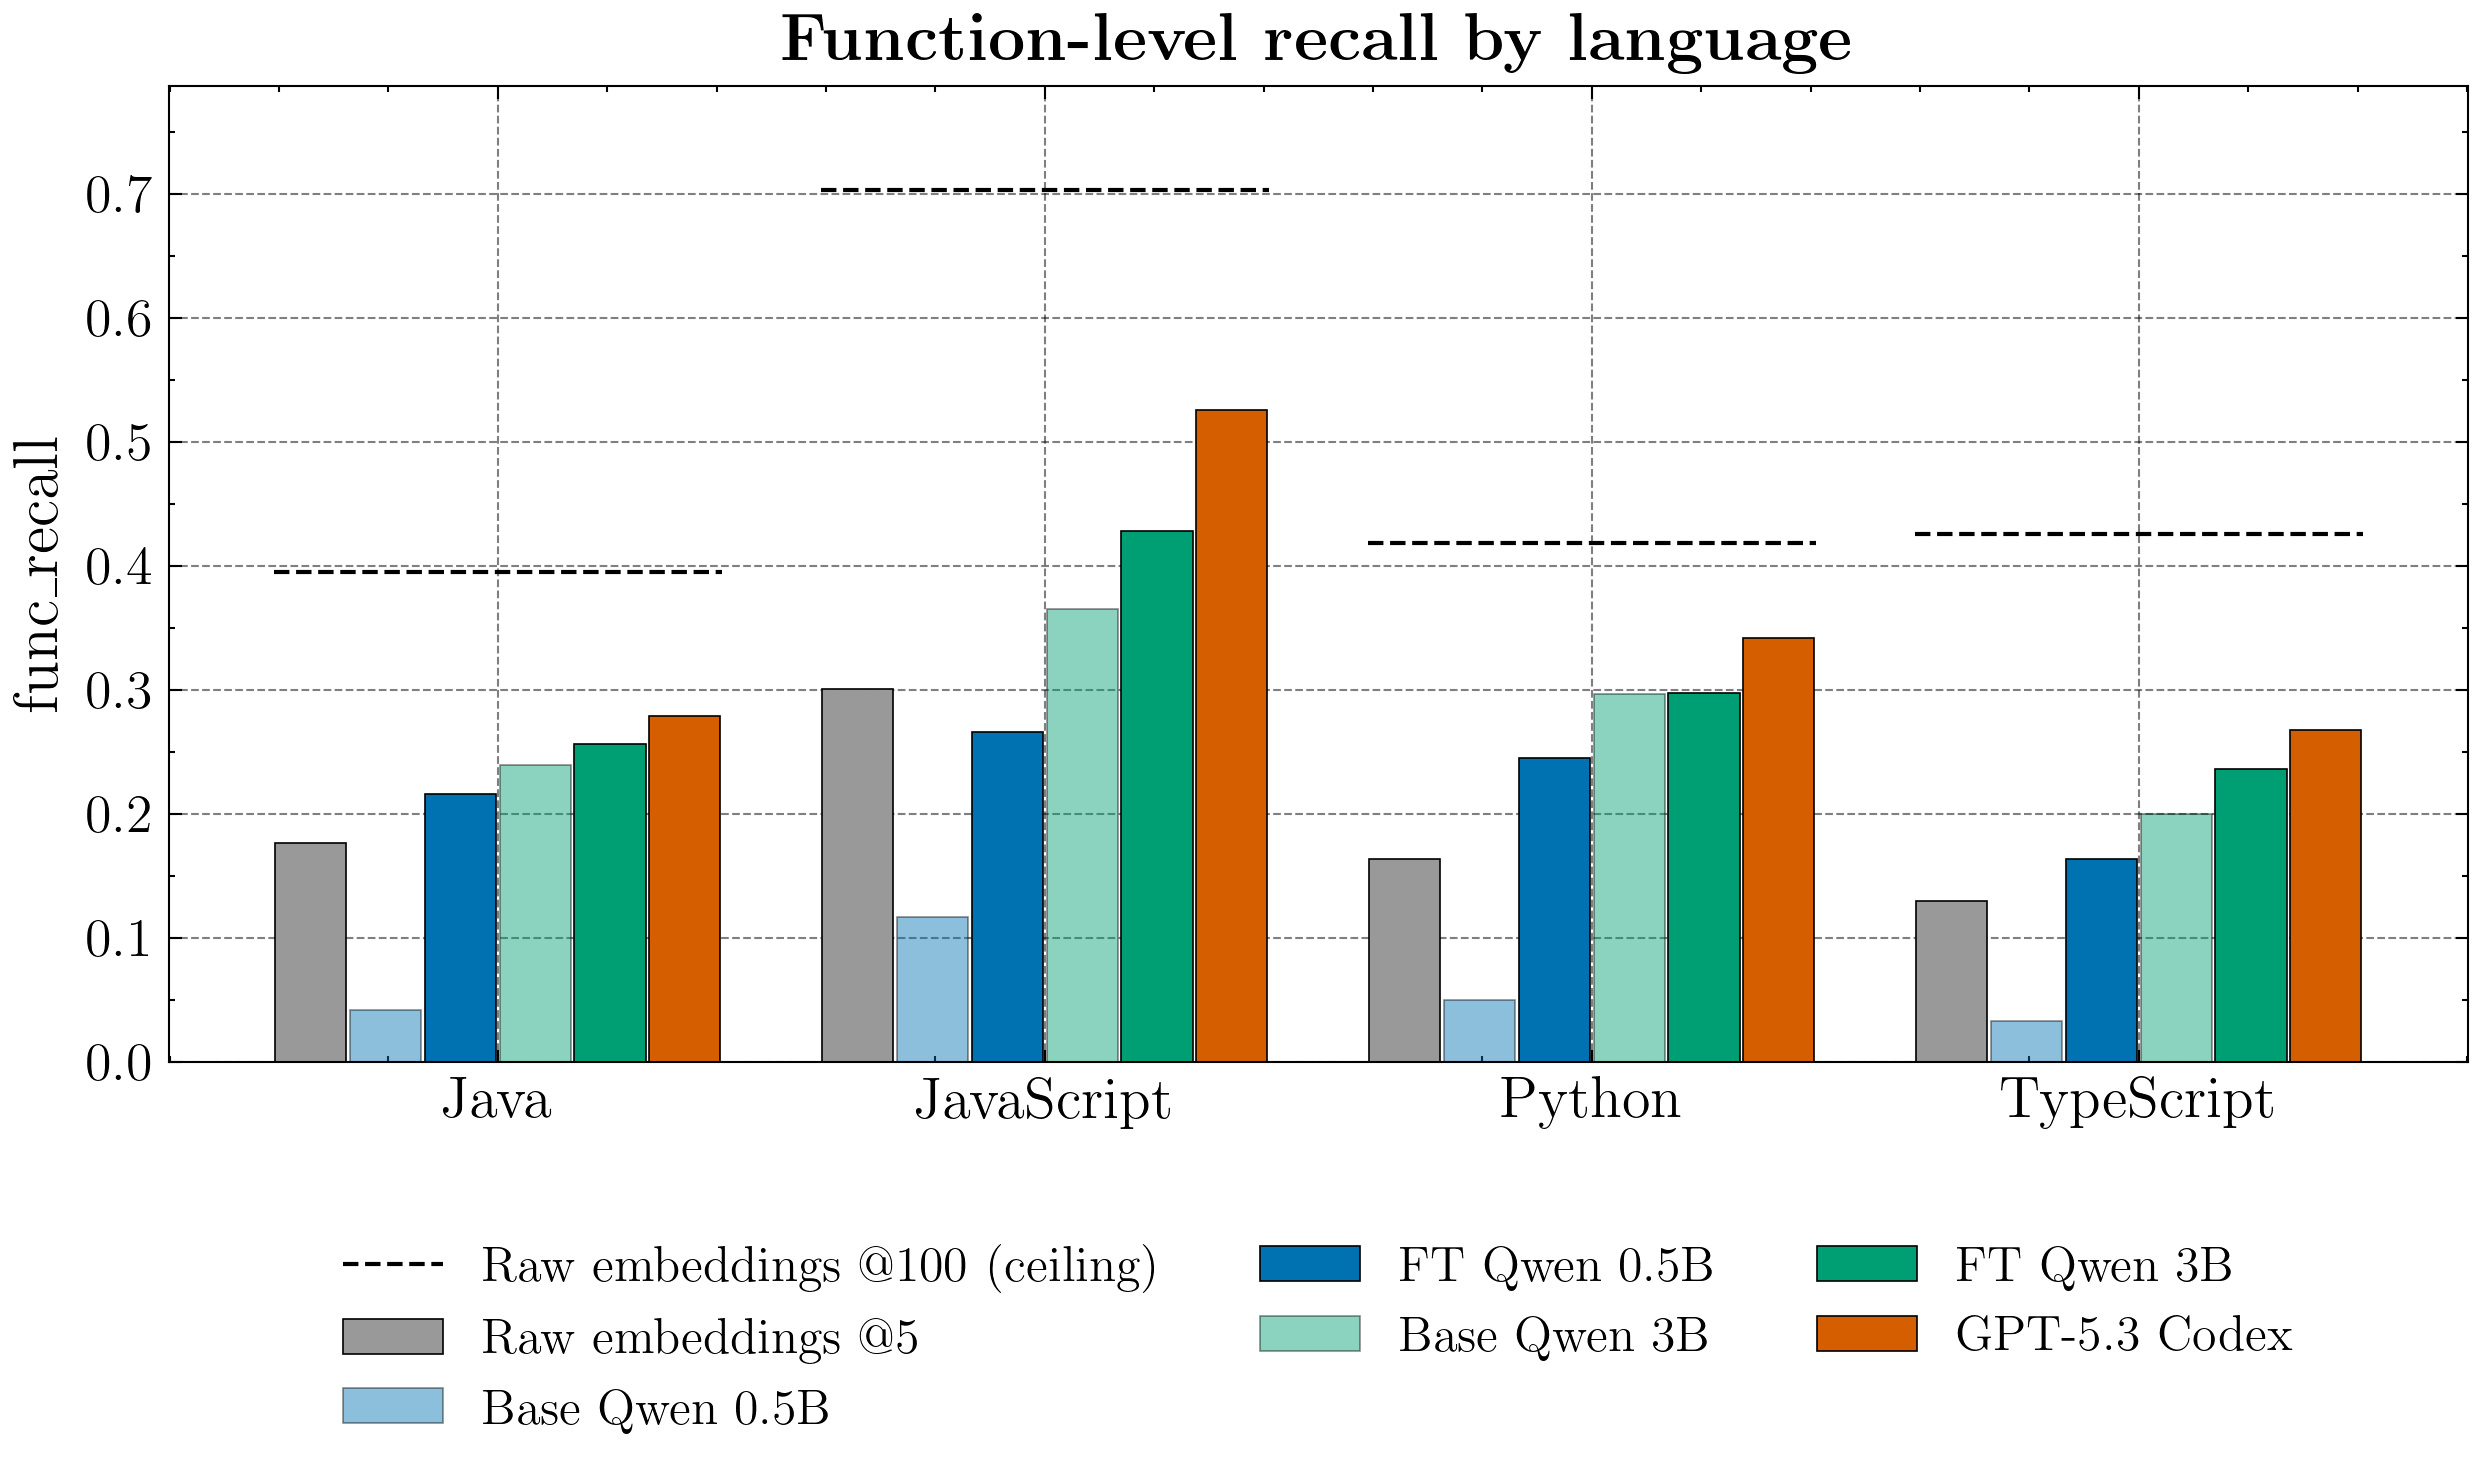
\includegraphics[width=\columnwidth]{imgs/reranker_func_recall.png}
\caption{Per-language function-level recall on SWE-PolyBench
under a windowed scorer protocol (pool size
$\text{PS}{=}100$, candidate window $K{=}20$, top-$L{=}5$). The
dashed line is the retrieval ceiling at $\text{PS}{=}100$.
Comparisons include the raw embedding ranker at $L{=}5$, base
and fine-tuned Qwen2.5-Coder 0.5B/3B-Instruct, and GPT-5.3
Codex. The fine-tuned 3B scorer dominates the 0.5B variants
and trails GPT-5.3 Codex by $2$--$10$ points across languages;
JavaScript shows the largest residual gap, where GPT-5.3 Codex
benefits most from its longer context.}
\label{fig:scorer-func-recall}
\end{figure}

\paragraph{End-to-end results on SWE-PolyBench.}
Table~\ref{tab:swepoly-java-python} reports end-to-end Recall@5
and Accuracy@5 on the SWE-PolyBench Java and Python splits,
where Accuracy@$K := \frac{1}{N}\sum_i \mathbb{1}[G_i \subseteq
\hat{L}_i]$ is the fraction of issues for which \emph{every}
gold function is recovered (i.e.\ perfect recall), comparing the scaffolding without graph
exploration (Step~B disabled) against the full scaffolding with
our fine-tuned scorer. The full scaffolding improves both
metrics on both languages: on Java, GPT-5.3 Codex gains $+5$
recall and $+5$ accuracy points; on Python, Qwen3-Coder-30B
gains $+5$ recall and $+4$ accuracy points and overtakes the
GPT-5.3 Codex baseline. Token consumption stays comparable to
the no-graph variant, so the gains come essentially free of
extra compute.

The Python ordering deserves a closer look: Qwen3-Coder-30B
overtakes GPT-5.3 Codex not because of better retrieval, but
because GPT-5.3 Codex triggers the early-stop flag too
aggressively. On the $120$ Python issues where GPT-5.3 Codex
ended the loop early, its Recall@5 is $0.476$, whereas Qwen3
running the full round budget on the \emph{same} issues reaches
$0.529$ --- a $+5.3$-point gap that comes entirely from the
exploration rounds GPT chose to skip. The recall deficit is
therefore a confidence-calibration artefact at Step~C, not a
shortcoming of the scorer or the retriever.

\begin{table*}[t]
\centering
\small
\setlength{\tabcolsep}{5pt}
\renewcommand{\arraystretch}{1.05}
\caption{Retrieval performance on SWE-PolyBench Java and Python
under two Step-C agents (GPT-5.3 Codex and
Qwen3-Coder-30B-A3B-Instruct). Recall@5 and Accuracy@5 (perfect
recall) are reported after filtering out instances with empty
function-level GT and using denominator
$|GT \cap \mathrm{graph\_functions}|$. ``--'' marks a run we
have not executed. Token consumption is the total tokens per
issue (tokens/call $\times$ \#calls), averaged across kept
instances.}
\label{tab:swepoly-java-python}
\begin{subtable}{0.49\textwidth}
\centering
\setlength{\tabcolsep}{4pt}
% \caption*{Java (kept $= 158$ / $165$)}
\caption*{Java}
\begin{tabular}{lccc}
\toprule
Model                          & Rec@5 & Acc@5 & Tokens (k) \\
\midrule
\multicolumn{4}{l}{\emph{w/o graph (Step B disabled)}} \\
GPT-5.3 Codex                  & $0.38$ & $0.22$ & $21.7$ \\
Qwen3-Coder-30B-A3B            & $0.35$ & $0.20$ & $27.8$ \\
\midrule
\multicolumn{4}{l}{\emph{Full, ours (Qwen2.5-Coder-3B scorer)}} \\
GPT-5.3 Codex                  & $\mathbf{0.43}$ & $\mathbf{0.27}$ & $\mathbf{19.1}$ \\
Qwen3-Coder-30B-A3B            & $0.37$ & $0.20$ & $26.8$ \\
\bottomrule
\end{tabular}
\end{subtable}
\hfill
\begin{subtable}{0.49\textwidth}
\centering
\setlength{\tabcolsep}{4pt}
% \caption*{Python (kept $= 182$ / $199$)}
\caption*{Python}
\begin{tabular}{lccc}
\toprule
Model                          & Rec@5 & Acc@5 & Tokens (k) \\
\midrule
\multicolumn{4}{l}{\emph{w/o graph (Step B disabled)}} \\
GPT-5.3 Codex                  & --     & --     & --     \\
Qwen3-Coder-30B-A3B            & $0.40$ & $0.29$ & $38.1$ \\
\midrule
\multicolumn{4}{l}{\emph{Full, ours (Qwen2.5-Coder-3B scorer)}} \\
GPT-5.3 Codex                  & $0.42$ & $0.31$ & $\mathbf{30.9}$ \\
Qwen3-Coder-30B-A3B            & $\mathbf{0.45}$ & $\mathbf{0.33}$ & $46.4$ \\
\bottomrule
\end{tabular}
\end{subtable}
\end{table*}

% \subsection{Does the Coverage Term Help?}
% \label{sec:ablation}
% - The key ablation: lambda = 0 (BCE only) vs lambda = 0.2
%   (BCE + coverage). Report the recall@L delta -- this is THE
%   objective-paper result.
% - Diagnostics (one line here, rest -> appendix): mean p on
%   gold vs non-gold; fraction of golds landing in the top-L.
%   (~0.2 page)

% \subsection{Efficiency and Scaling}
% \label{sec:efficiency}
% - FIGURE 2: token cost. Per-call and total tokens vs
%   OpenHands; bounded vs unbounded trajectory length; wall-
%   clock saved. Plot with SciencePlots (project .venv, PDF).
% - Scaling: recall@L vs number-of-gold-nodes and vs gold
%   graph-spread -- a widening margin over a ranking baseline
%   (SweRank). This is the make-or-break analysis.
% - TRIAGE: 4 pages cannot comfortably hold both an efficiency
%   figure and a scaling figure. Put ONE in the body (the
%   scaling figure is the stronger novelty signal) and move the
%   other to Appendix C, or render efficiency as a small table.
%   (~0.25-0.3 page)

\section{Discussion and Conclusion}
\label{sec:conclusion}

\paragraph{Discussion.}
The picture across SWE-Bench Verified
(Table~\ref{tab:verified}) and SWE-PolyBench
(Table~\ref{tab:swepoly-java-python},
Figure~\ref{fig:scorer-func-recall}) is consistent. First, a
bounded-context scaffolding closes most of the gap left by the
first-stage retriever: every LLM-driven configuration we tried
exceeds the $\approx0.35$ Recall@5 ceiling of the zero-shot
ranker. Second, graph exploration (Step~B) is the largest single
lever, lifting recall and accuracy on every model and language
while keeping per-call context short. Third, a small fine-tuned
scorer is enough to drive the full scaffolding: a
Qwen2.5-Coder-3B scorer matches Qwen3-Coder-30B-A3B under the
same scaffolding on Verified at roughly an order of magnitude
lower token cost ($35.6$k vs $\geq 198$k tokens per issue), and
pairs with a 30B Step-C agent to set the best Python numbers on
SWE-PolyBench.
Token consumption tracks the call count rather than the model
size, so larger Step-C agents do not pay a context tax for using
our scorer.

\paragraph{Key takeaways.}
(i) Localization scales better through scaffolding structure
than through model size: a 3B scorer plus a 30B agent under our
loop beats a 30B agent alone. (ii) Graph-aware exploration is
cheap because the scorer sees short neighborhood windows rather
than the full pool; the cost of an extra step is small compared
to the recall it recovers. (iii) Supervised training is
sufficient for the scorer because the per-round shaping signal
telescopes to end-to-end Recall@$K$, so no policy-gradient
machinery is needed for the inner loop.

\paragraph{Conclusion.}
We cast code localization as sequential set-coverage on a code
graph and built a bounded-cost, multi-round, multi-agent
scaffolding around that view. The round structure exposes a
dense per-round target whose optimum coincides with end-to-end
Recall@$K$, which lets a small open scorer be trained by
ordinary supervised learning rather than sparse-reward RL. The
resulting Qwen2.5-Coder-3B scorer makes the full scaffolding
competitive with GPT-5.3 Codex on SWE-Bench Verified and on
SWE-PolyBench Java and Python, at a fraction of the token cost.
Stop-timing and cross-round coordination remain natural
candidates for a light-weight RL stage on top of the supervised
scorer; we leave that to future work.


% Limitations is required by ACL, is unnumbered, and does not
% count toward the 4-page main-content limit.
\section*{Limitations}
\label{sec:limitations}

\paragraph{Partial multilingual coverage.}
Our end-to-end scaffolding results on SWE-PolyBench
(Table~\ref{tab:swepoly-java-python}) cover only the Java and
Python splits at submission time; the JavaScript and TypeScript
end-to-end runs are not yet complete. The standalone scorer
evaluation (Figure~\ref{fig:scorer-func-recall}) does span all
four languages, so the trained scorer itself has been measured
broadly, but the full Step-A/B/C pipeline numbers for
JavaScript and TypeScript are pending.

\paragraph{Benchmark scope.}
All evaluations are on SWE-Bench-family benchmarks
(SWE-Bench Verified and SWE-PolyBench). These cover
human-curated GitHub issues drawn mostly from popular
open-source libraries; generalization to private-codebase
distributions, proprietary languages, or non-bug-fix
maintenance tasks (refactors, feature additions) is untested.

\paragraph{Graph construction is assumed away.}
The scaffolding requires a pre-built code graph $\mathcal{G}$.
We reuse the graphs released with prior work and construct new
ones with the same pipeline (Appendix~\ref{app:graph}), but the
construction cost, the failure modes for languages with weaker
Tree-sitter coverage, and the sensitivity of recall to graph
quality are not studied here. A noisy or incomplete graph is a
silent failure mode that this paper does not characterise.

\paragraph{Surrogate coverage term.}
The listwise term $\mathcal{L}_{\text{cov}}$ in~\eqref{eq:cov}
is a differentiable softmax surrogate, not the exact
(non-differentiable) set-coverage objective. Our argument
guarantees that the dense per-round target shares the same
optimum as end-to-end Recall@$K$; whether $\mathcal{L}_{\text{cov}}$
attains that optimum exactly, rather than only approximating it,
is not proven.

\paragraph{Single scorer backbone.}
We instantiate the scorer only on Qwen2.5-Coder-3B-Instruct
(with a 0.5B variant reported as an ablation). How the recipe
scales to other base families (Llama-Coder, DeepSeek-Coder,
non-Coder instruction models) or to substantially larger
adapters is not evaluated.

\paragraph{Stop-timing and cross-round coordination.}
The scaffolding always runs to the round budget or pool
exhaustion; an early-stop hook is left for an RL stage that we
do not train or evaluate in this paper. Likewise, cross-round
coordination between the scorer and the agent uses a fixed
protocol and is not learned. Both are natural targets for a
follow-up that adds a thin RL layer on top of the supervised
scorer.


% TEMP: \nocite{*} lists every custom.bib entry so the outline
% skeleton compiles a References section. Remove it once the
% sections cite sources with \citep.
\nocite{*}
\bibliography{custom}

\appendix
% ============================================================
% OUTLINE -- Appendix     unlimited pages; supplementary only.
% Nothing here is required to follow the 4-page main text.
% Sections become A, B, C, ... under \appendix (set in
% acl_latex.tex).
% ============================================================

\section{Proof of the Telescoping Identity}
\label{app:proof}
% - Full statement and proof that sum_t r_t = recall@K(\hat{L}_R) -
%   recall@K(\hat{L}_0) under equal add/drop weights, and that
%   potential-based shaping \citep{ng1999policy} leaves the
%   optimal policy invariant -- so the dense objective and the
%   recall@K optimum coincide.
% - Regret view: Case 1 (a gold-for-gold swap) has regret 0;
%   Case 2 (a non-gold kept over a gold) has regret 1.

\section{Code Graph Construction}
\label{app:graph}

The scaffolding's neighborhood expansion
(Section~\ref{sec:scaffold}, Step~B) walks a per-repository
code graph $\mathcal{G}{=}(V,E)$. We follow the four-edge
schema of \citet{chen2025locagent} as implemented in
\citet{chaudhari2025spider}, summarised here for completeness.

For each repository the graph is built from the source files
written in the repository's primary language; files in
secondary languages are ignored. Nodes represent code entities
at four granularities (directory, file, class, and function),
and edges encode four structural relations: a \textit{contains}
edge linking each container to the code units it declares, an
\textit{invokes} edge between a function and each function it
calls, an \textit{imports} edge between a file and each module
it imports, and an \textit{inherits} edge between a class and
each parent class it extends. Every non-directory node stores
its source text alongside its identifier, so the model can see
code when a node is shown.

We extract Python source files with the standard \texttt{ast}
module and Java, JavaScript, and TypeScript files with
Tree-sitter\footnote{\url{https://github.com/tree-sitter}}. The
traversal of the repository's directory tree adds directory
nodes for navigation, skips files that contain no class or
function definition, and emits one node per declared entity
together with its containment, call, import, and inheritance
edges. Multi-file class definitions and the more flexible
declaration patterns of the non-Python languages are handled
with language-specific Tree-sitter queries; we refer to
\citet{chaudhari2025spider} for the full list of cases. Graphs
are constructed on demand at the start of a localization run
and reused across the rounds.

For the experiments in Section~\ref{sec:experiments}, we use
the graphs released with \citet{chaudhari2025spider} for
SWE-PolyBench and SWE-Bench Verified, and construct graphs from
scratch for the SWE-Bench Lite dev split with the same
pipeline.

\section{Scorer Training Details}
\label{app:details}

This appendix complements Section~\ref{sec:training} with the
hyperparameters and procedural details that we omit from the main
body.

\paragraph{Group construction.}
For each issue, every ground-truth function that falls inside the
retriever's top-$N$ pool is included as a positive; the group is
then completed to size $M$ with non-relevant candidates. Negatives
are drawn with a stratified strategy: a fixed fraction is taken as
top-ranked hard negatives, and the remaining slots are filled by
partitioning the rest of the pool into equal-width rank bins and
sampling one negative per bin. Each group therefore exposes the
model to shallow, mid- and deep-pool negatives, which empirically
prevents the calibration drift on deep-pool non-relevant candidates
we observed under top-only hard-negative sampling. Negatives are
re-sampled at the start of every epoch, so depth coverage widens
monotonically across training.

\paragraph{Optimization.}
The adapter is trained in bfloat16 with FlashAttention-2 and
activation checkpointing on the backbone. AdamW is used with the
schedule of Table~\ref{tab:hparams}; gradients are accumulated over
$8$ groups before each optimizer step and clipped to unit norm. All
$M$ candidates of a group are forwarded under autograd in a single
optimizer iteration so that the listwise term in~\eqref{eq:cov}
backpropagates jointly across the group.

\paragraph{Distributed training.}
Training is data-parallel across GPUs via Hugging Face Accelerate.
At the start of each epoch the shuffled issue list is sharded into
disjoint contiguous slices --- one per rank --- and each rank
builds its own training groups independently. Because issues whose
ground-truth functions fall outside the retriever pool are dropped,
the per-rank post-filter group counts are reduced with a
min-collective to keep DDP collectives aligned. LoRA gradients are
small relative to the backbone, so all-reducing them on every
backward is inexpensive and we do not shard the model.

\paragraph{Evaluation during training.}
After each epoch the current adapter is evaluated on a fixed
held-out subset of validation issues using the same windowed
top-$K$ procedure as inference: candidates are scored in sliding
windows over the top-$N$ pool, the global top-$K$ by score is
selected, and function- and file-level $\text{recall}@K$ are
reported. Best-epoch selection on this validation metric determines
the adapter shipped for the test-time evaluation in
Section~\ref{sec:experiments}.

\paragraph{Prompt format.}
The training-time prompt format matches the inference scorer's
format exactly, including the assistant-turn template and the
position at which the \textsc{yes}/\textsc{no} logits are read.
Mismatches between train- and test-time prompts silently shift the
score distribution and are the most common source of regression
when porting the adapter to a new backbone.

\begin{table}[h]
\centering
\small
\caption{Scorer fine-tuning hyperparameters. The same
configuration is used for the BCE-only ($\lambda{=}0$) ablation
and the main BCE+coverage ($\lambda{=}0.2$) runs.}
\label{tab:hparams}
\setlength{\tabcolsep}{4pt}
\renewcommand{\arraystretch}{1.05}
\begin{tabular}{ll}
\toprule
\textbf{Component} & \textbf{Value} \\
\midrule
Backbone               & Qwen2.5-Coder-3B-Instruct \\
                       & \citep{hui2024qwen25codertechnicalreport} \\
Precision              & bfloat16, FlashAttention-2 \\
Adapter                & LoRA, $r{=}4$, $\alpha{=}32$, dropout $0.05$ \\
LoRA targets           & $\{q,k,v,o\}_{\text{proj}}$, \\
                       & $\{\text{gate},\text{up},\text{down}\}_{\text{proj}}$ \\
Score readout          & $s = \ell(\text{yes}) - \ell(\text{no})$ \\
                       & at final prompt position \\
Group size $M$         & $20$ candidates per issue \\
Issue / code trunc.    & $3072$ / $1024$ tokens \\
Negative sampling      & $40\%$ top hard negatives; \\
                       & remainder one-per-bin across pool; \\
                       & re-sampled each epoch \\
BCE class weights      & $w_{+}{=}w_{-}{=}1$ \\
Coverage weight        & $\lambda{=}0.2$ (main); $\lambda{=}0$ (ablation) \\
Optimizer              & AdamW \\
Learning rate          & $1{\times}10^{-4}$, cosine, $3\%$ warm-up \\
Grad. accumulation     & $8$ groups per step \\
Grad. clipping         & max norm $1.0$ \\
Epochs                 & $5$ \\
Retriever pool $N$     & $500$ \\
Train / val split      & $95\%/5\%$ of issues, fixed seed \\
\bottomrule
\end{tabular}
\end{table}

\section{Additional Results}
\label{app:results}

The figures below complement the function-level scorer
evaluation reported in
Section~\ref{sec:main-results} (Figure~\ref{fig:scorer-func-recall}).
Both use the same windowed protocol on SWE-PolyBench: the
first-stage retriever returns the top $\text{PS}{=}100$
candidates, the scorer ranks a window of $K{=}20$, and the
top-$L{=}5$ by score are selected.

\begin{figure*}[t]
\centering
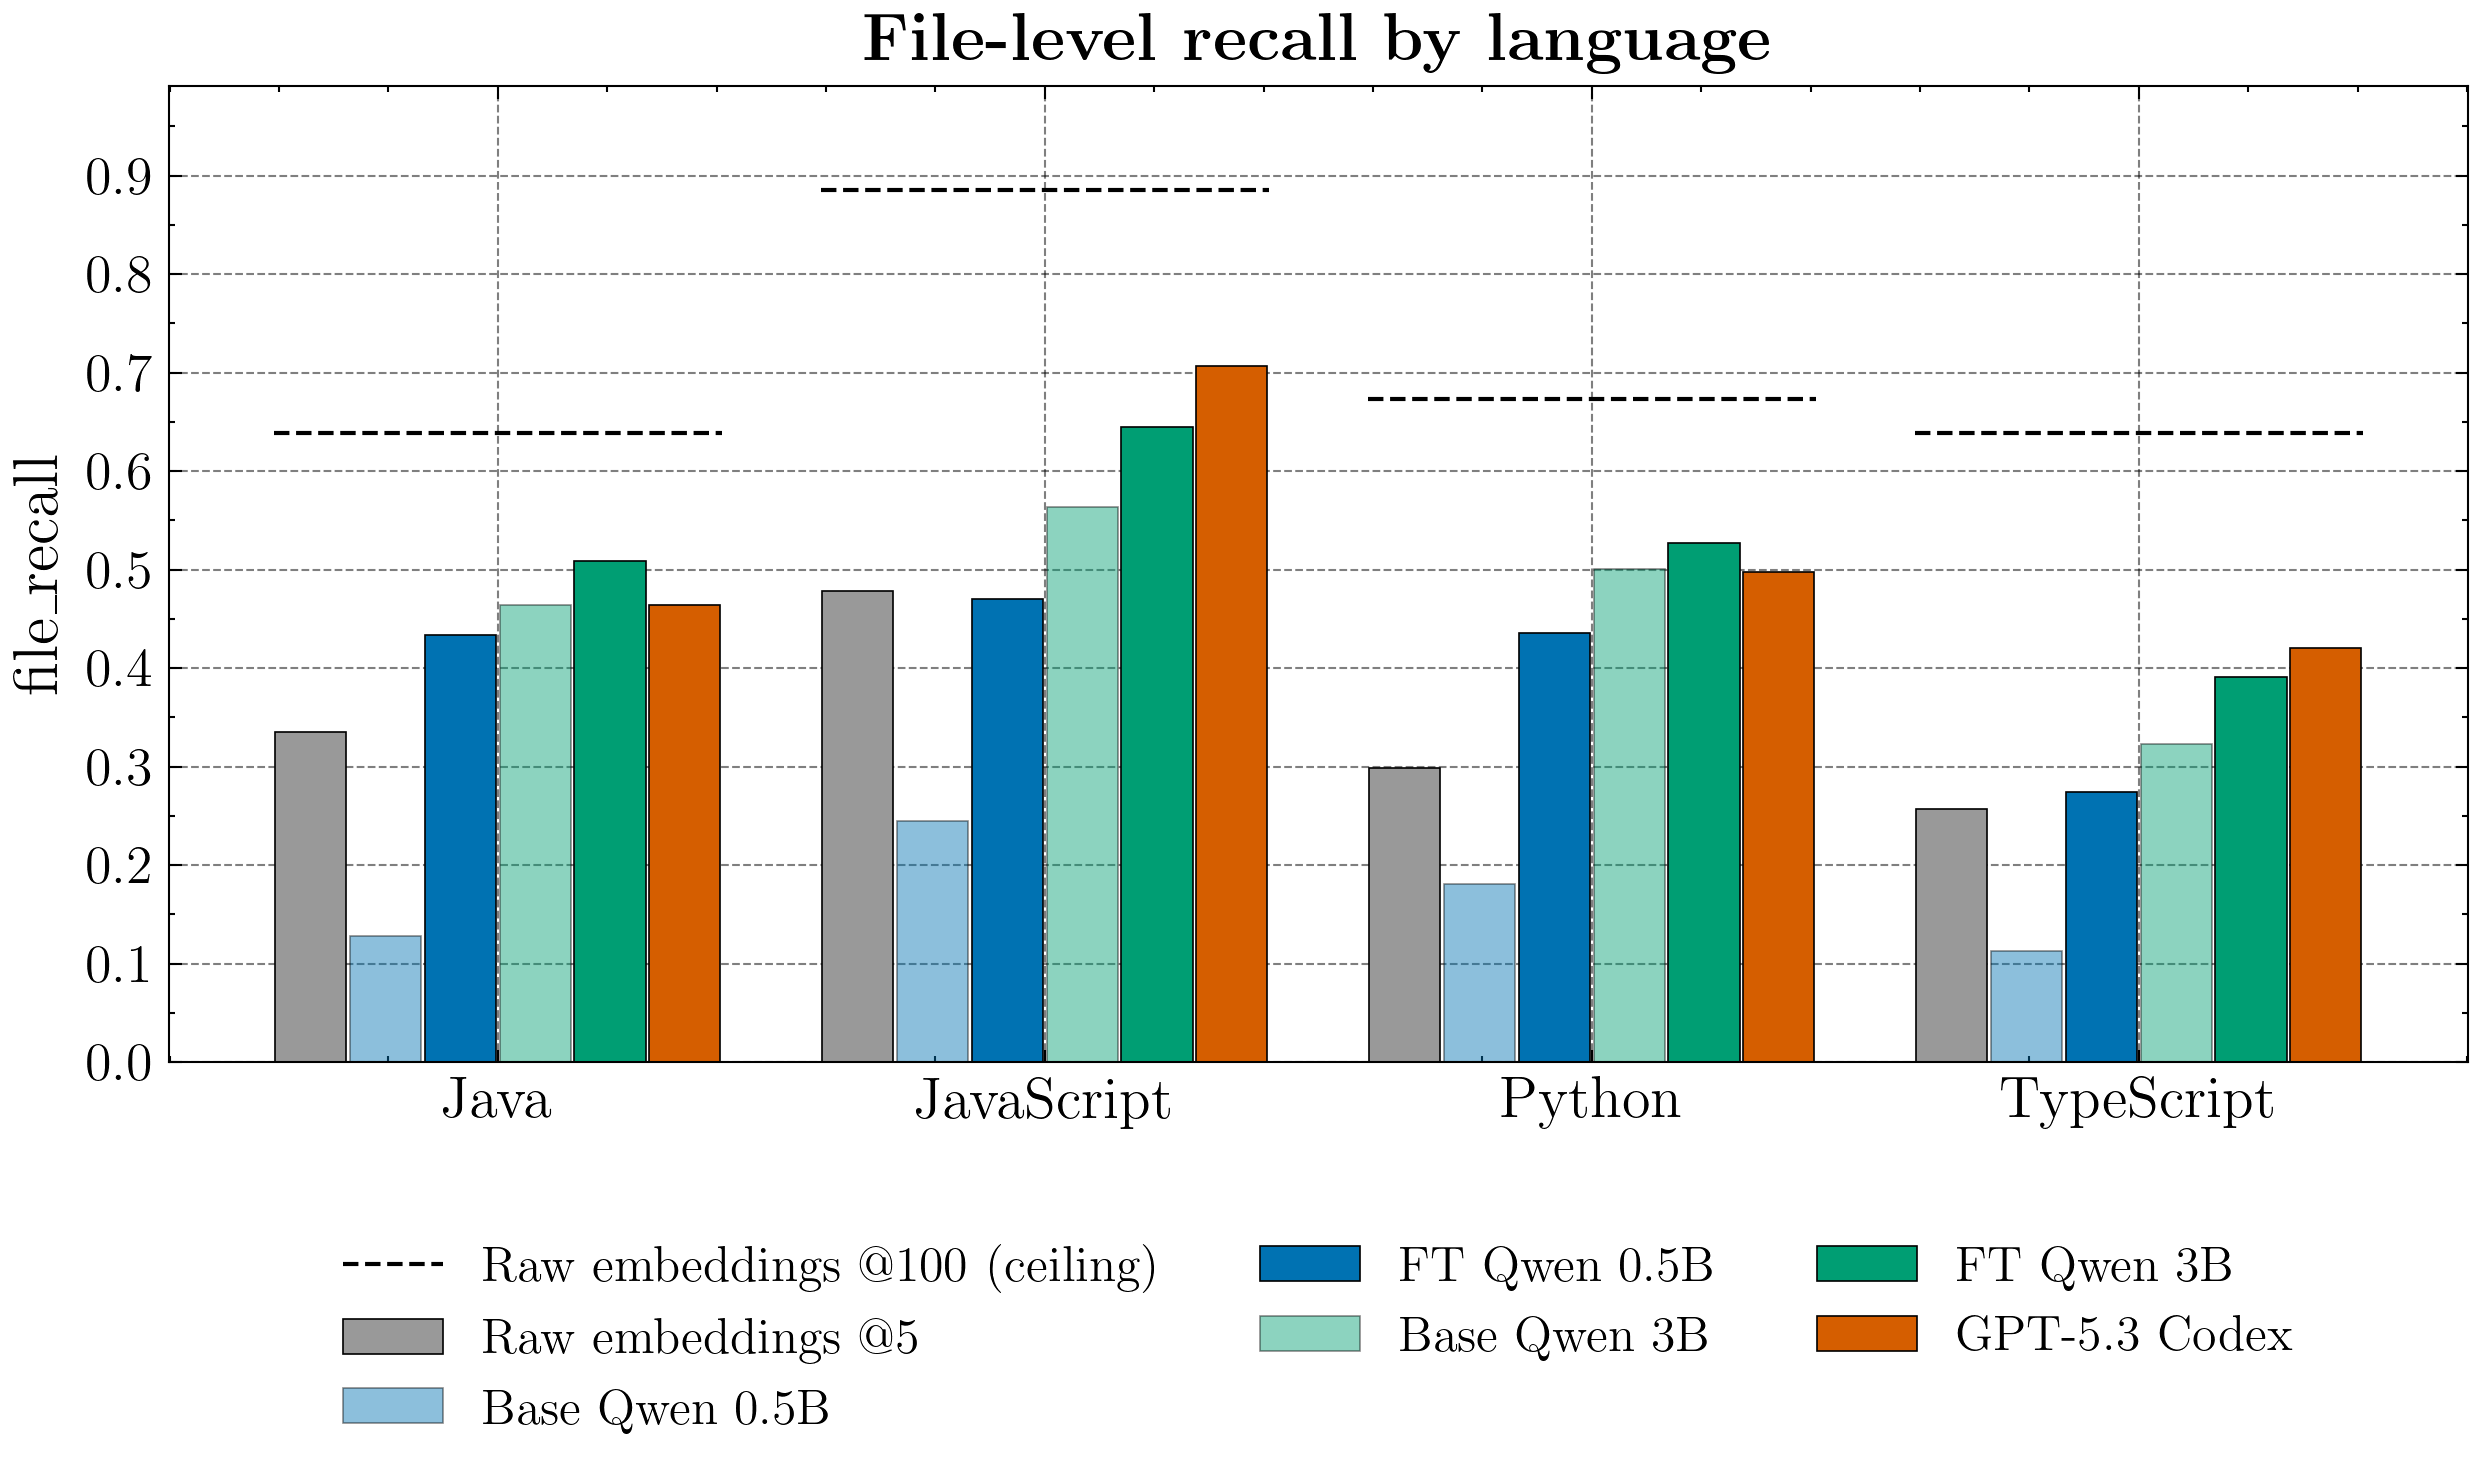
\includegraphics[width=0.85\textwidth]{imgs/reranker_file_recall.png}
\caption{Per-language file-level recall on SWE-PolyBench under
the windowed protocol of Figure~\ref{fig:scorer-func-recall}.
The dashed line marks the retrieval ceiling --- the recall
achievable if the gold function set lies in the top-$100$
retriever pool. The fine-tuned 3B scorer (FT Qwen 3B) matches
or exceeds GPT-5.3 Codex on Java and Python and tracks it within
a few points on JavaScript and TypeScript.}
\label{fig:scorer-file-recall}
\end{figure*}

\begin{figure*}[t]
\centering
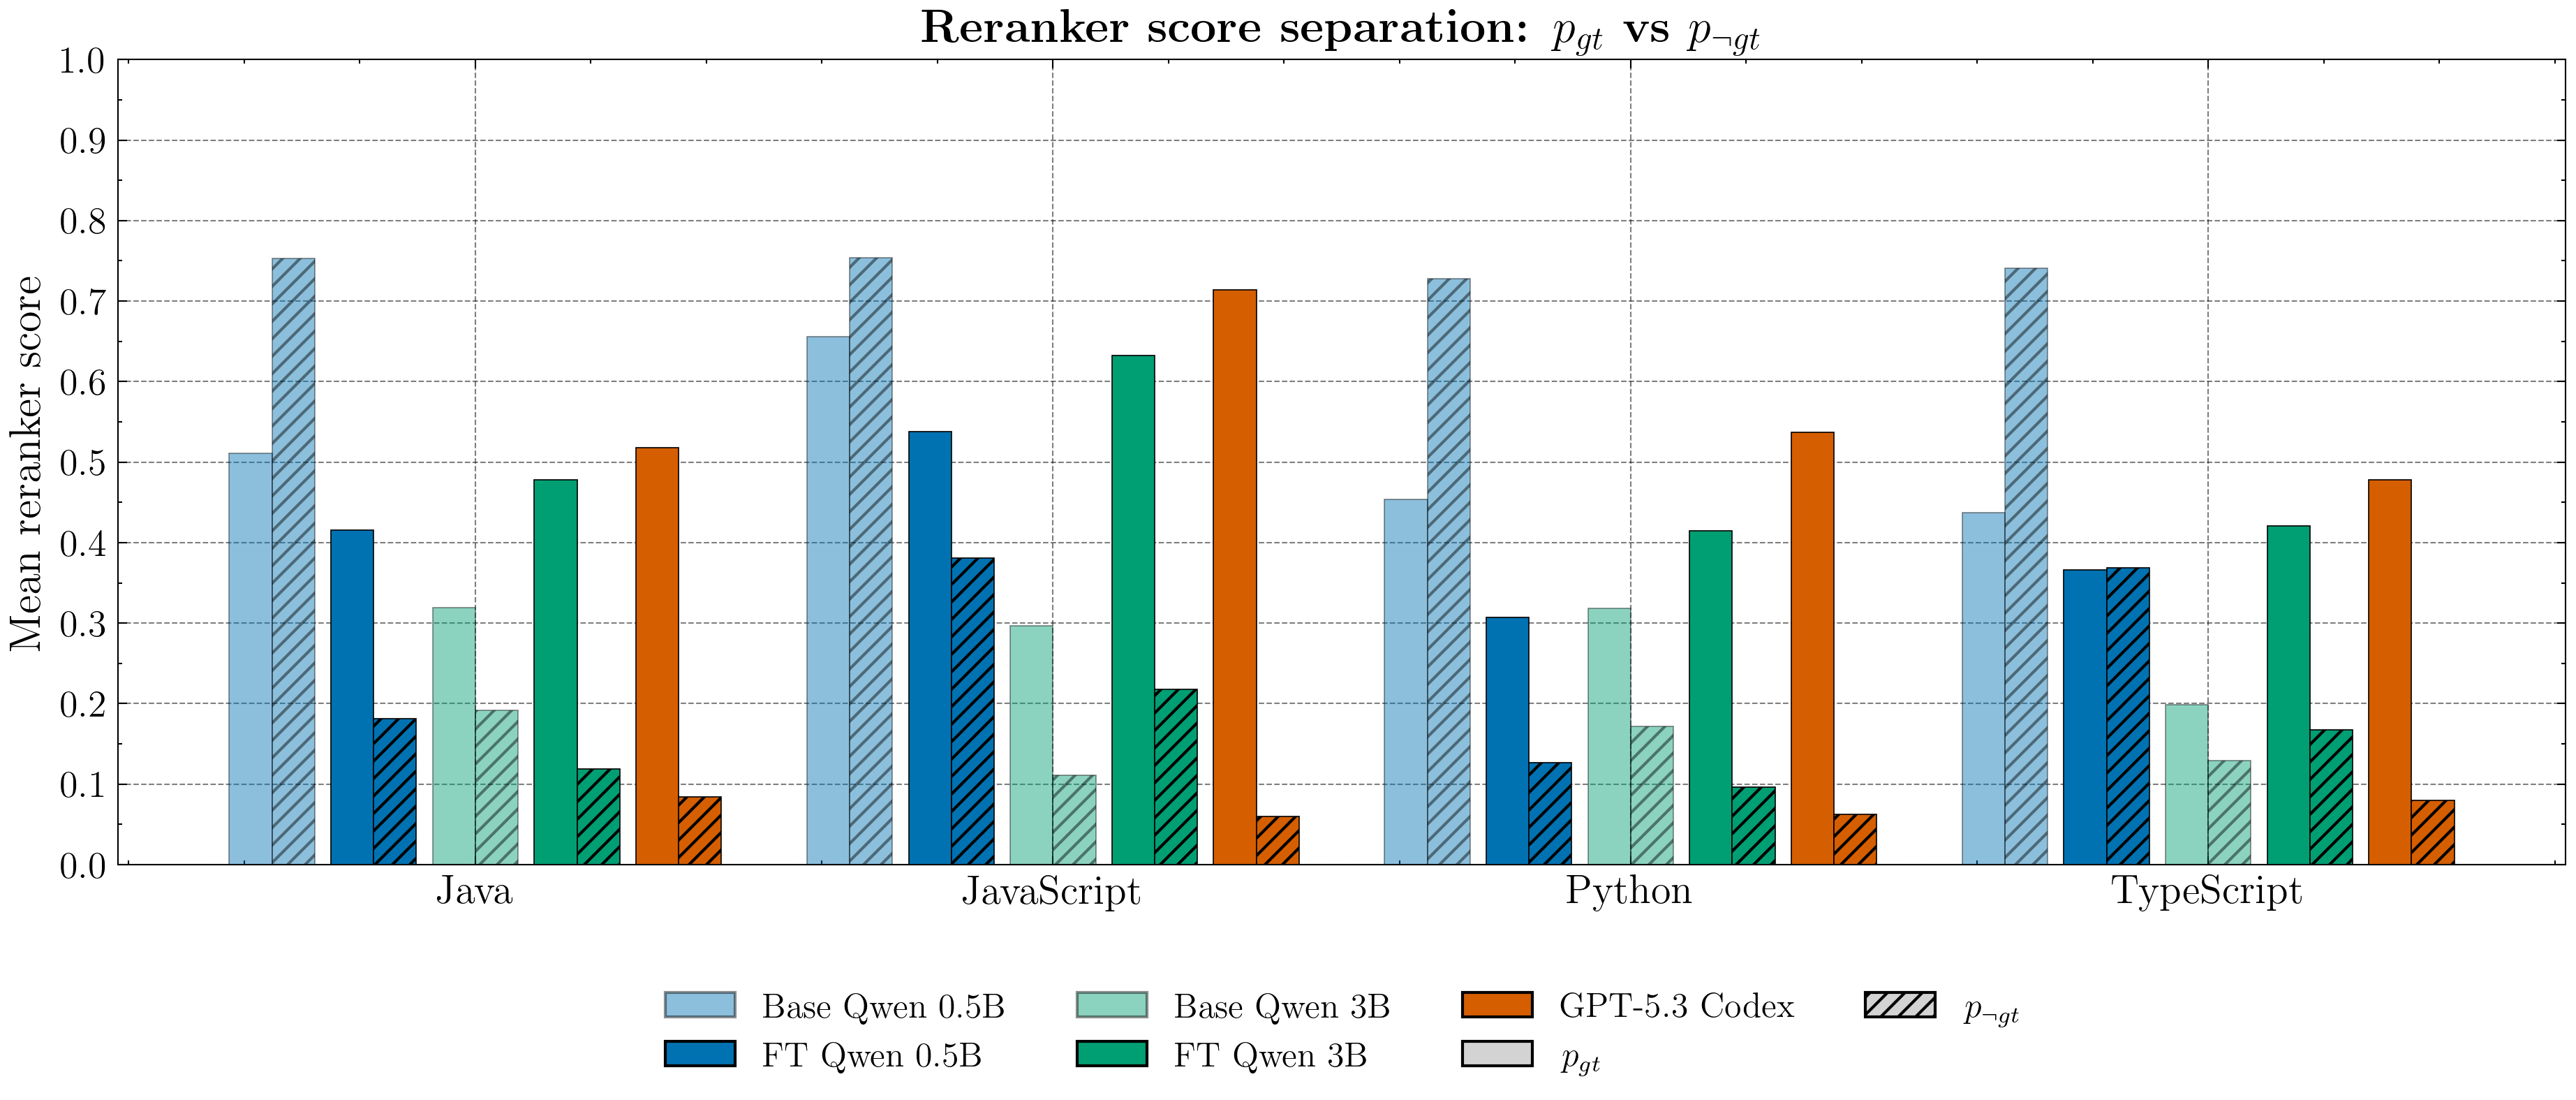
\includegraphics[width=0.85\textwidth]{imgs/reranker_score_separation.png}
\caption{Mean score on ground-truth candidates
($p_{gt}$, filled bars) vs.\ non-relevant candidates
($p_{\neg gt}$, hatched bars), averaged per language under the
same windowed protocol. A wider gap indicates better
discrimination between gold and non-gold. Fine-tuning widens
the separation at every model size: the base 0.5B model is
actively mis-calibrated --- it assigns $p_{\neg gt} > p_{gt}$
in every language --- whereas the fine-tuned 3B variant
achieves a separation comparable to GPT-5.3 Codex, with
$p_{gt}$ above $p_{\neg gt}$ by a margin of $0.25$--$0.45$.}
\label{fig:scorer-score-separation}
\end{figure*}

\section{AI Disclosure}
\label{app:ai}
% - The ACL-required statement of AI-tool usage. Generate it
%   with the academic-paper `disclosure` mode once drafting is
%   complete.


\end{document}
